\documentclass{lecturenotes}

\title[Föreläsningsanteckningar EDA016, 2015]{EDA016 Programmeringsteknik för D}
\subtitle{Läsvecka 1: Introduktion}
\author{Björn Regnell}
\institute{Datavetenskap, LTH}
\date{Lp1-2, HT 2015}
 
\begin{document}
 
\frame{\titlepage}
\section[Vecka 1: Introduktion]{Introduktion}

%%%%%%%%%%%%%%%%%%%%%%%%%%%%%%%%%%%%%%
\subsection{Om denna kurs}

\frame{\tableofcontents}

%%%
\frame{\frametitle{Vad och hur?}\begin{itemize}
\item \emph{Vad} ska du lära dig?
\begin{itemize}
\item Grundläggande principer för programmering
\item Konstruktion av enkla algoritmer
\item Tänka i abstraktioner
\item Imperativ och objektorienterad programmering
\item Programspråket Java
\item Utvecklingsmiljön Eclipse: implementera, testa, felsöka
\end{itemize}
\item \emph{Hur} ska du lära dig?
\begin{itemize}
\item Genom praktiskt eget arbete: Lära genom att göra!
\item Genom studier av kursens teori: Skapa förståelse
\item Genom samarbete med dina kurskamrater
\end{itemize}
\end{itemize}}

%%%
\frame{\frametitle{Kurslitteratur}
\begin{columns}
\begin{column}{0.6\textwidth}
\begin{itemize}
\item ''Objektorienterad programmering och Java" av Per Holm
\item Kurskompendium med övningar och laborationer
\item Bokpaket säljs på KFS \\John Ericssons väg 4 \url{http://www.kfsab.se/}
\end{itemize}
\end{column}
\begin{column}{0.5\textwidth}
\centering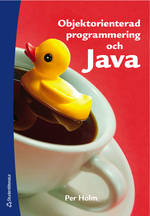
\includegraphics[width=0.5\textwidth]{img/ankbok.jpg}
\end{column}
\end{columns}
}

%%%
\frame{\frametitle{Personal}\footnotesize
\begin{description}
\item [\bfseries Kursansvarig:] ~\\Björn Regnell, bjorn.regnell@cs.lth.se
\item [\bfseries Kurssekreterare:]  ~\\Lena Ohlsson \\Exp.tid 09.30 - 11.30 samt 12.45 - 13.30
\item [\bfseries Handledare:] ~\\
Gustav	Cedersjö,	Doktorand\\
Maj	Stenmark,	Doktorand\\
Anton	Klarén,	D09\\
Maria	Priisalu	, D11\\
Anders	Buhl,	D13\\
Erik	Bjäreholt,	D13\\
Fatima	Abou Alpha,	D13\\
Cecilia	Lindskog,	D14\\
Emma	Asklund,	D14\\
\end{description}
}

%%%
\frame{\frametitle{Kursmoment --- varför?}\footnotesize
\begin{itemize}
\item \textbf{Föreläsningar}: skapa översikt, ge struktur, förklara teori, svara på frågor, motivera varför
\item \textbf{Övningar}: bearbeta teorin med avgränsade problem som mestadels löses med papper  \& penna, förberedelse inför laborationerna
\item \textbf{Laborationer}: lösa programmeringsproblem praktiskt, obligatoriska uppgifter; lösningar redovisas för handledare
\item \textbf{Resurstider}: få hjälp med övningar och laborationsförberedelser av handledare
\item \textbf{Samarbetsgrupper}: grupplärande genom samarbete och dialog 
\item \textbf{Kontrollskrivning}: obligatorisk, diagnostisk, kamraträttad; kan ge samarbetsbonuspoäng till tentan
\item \textbf{Inlämningsupgift}: du visar att du kan skapa ett större program självständigt; redovisas för handledare
\item \textbf{Tenta}: Skriftlig tentamen utan hjälpmedel, förutom  \href{http://fileadmin.cs.lth.se/cs/Education/EDA016/general/quickref-booklet.pdf}{snabbreferens}.
\end{itemize}}

%%%
\frame{\frametitle{Nytt för i år }
Årets kurs är i flera avseende väsentligt annorlunda and förra årets upplaga, så lita inte på allt som era äldre kursare säger :) 
\begin{itemize}
\item Övningar blir resurstider i datorsal
\item Inlämningsuppgift utan skriftlig rapport
\item Samarbetskultur och grupplärande
\item Nya övningar 
\item Nya laborationer
\item Nya föreläsningar
\item Höjda ambitioner: Fler ska klara tentan med högre betyg och fler ska lära sig mycket mer än vad som ''råkar'' komma på tentan...
\end{itemize}
}

%%%
\frame{\frametitle{Detta är bara början... }
Exempel på efterföljande kurser som bygger vidare på denna:
\begin{itemize}
\item Årskurs 1
\begin{itemize}
\item Programmeringsteknik -- fördjupningskurs
\item Utvärdering av programvarusystem
\item Diskreta strukturer
\end{itemize}
\item Årskurs 2
\begin{itemize}
\item Objektorienterad modellering och design
\item Programvaruutveckling i grupp
\item Algoritmer, datastrukturer och komplexitet
\item Funktionsprogrammering
\end{itemize}
\end{itemize}
}

%%%
\frame{\frametitle{Förkunskapsenkät}}

%%%
\frame{\frametitle{Samarbetsgrupper}}

%%%
\frame{\frametitle{En typisk kursvecka i första läsperioden}
\begin{itemize}
\item Gå på föreläsningar måndag--tisdag
\item Jobba själv med boken, övningar, labbförberedelser
\item Träffas i samarbetsgruppen och hjälp varandra att förstå mer och fördjupa lärandet
\item Gå till resurstider och få hjälp och tips av handledare, onsdag--torsdag
\item Genomför obligatorisk laboration på fredagen
\end{itemize}
Se detaljerna och undantagen i \href{http://cs.lth.se/eda016/schema}{schemat i TimeEdit}
}

%%%
\frame{\frametitle{Resurstider}}

%%%
\frame{\frametitle{Laborationer}}

%%%
\frame{\frametitle{Att göra Vecka 1}
\begin{itemize}
\item Läs kursboken kapitel 1-3.2
\item Gör övning 1: Hello World, Hello Args, javac, editera--kompilera--exekvera--felsök, värden, uttryck variabler och tilldelning
\item Gör förberedelserna till laboration 1
\item Genomför laboration 1: Quiz --- träna på att editera, läsa, ändra och felsöka i färdig programkod
\item Funktionsprogrammering
\end{itemize}
}

%%%%%%%%%%%%%%%%%%%%%%%%%%%%%%%%%%%%%%
\subsection{Vad är programmering?}

%%%
\frame[plain]{
\centering\huge\bfseries\textcolor{blue}{Vad är programmering?}}

%%%
\frame[plain]{\frametitle{Programming unplugged}
\centering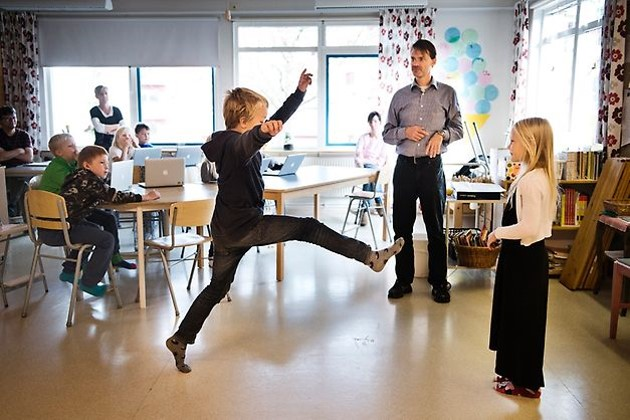
\includegraphics[width=1.0\textwidth]{img/unplugged.jpg}
}

\frame{\frametitle{Att skapa koden som styr världen}}

\frame{\frametitle{Vad är Java?}}

\frame{\frametitle{Vad är en kompilator och ett programspråk?}}

\frame{\frametitle{Utvecklingsverktyg}}

\frame{\frametitle{Vad är objektorientering?}
\begin{itemize}
\item Det finns många olika \href{https://en.wikipedia.org/wiki/Programming_paradigm}{programmeringsparadigm} (sätt att programmera på), till exempel:
\begin{itemize}
\item \textcolor{blue}{\bfseries imperativ programmering:} programmet är uppbyggt av sekvenser av olika satser som påverkar systemets tillstånd
\item \textcolor{blue}{\bfseries objektorienterad programmering:} en sorts imperativ programmering där programmet består av objekt som samlar data och operationer på data
\item \textcolor{blue}{\bfseries funktionsprogrammering:} programmet är uppbyggt av samverkande (matematiska) funktioner som undviker föränderlig data och tillståndsändringar  
\item \textcolor{blue}{\bfseries logikprogrammering:} programmet är uppbyggt av logiska uttryck som beskriver olika fakta eller villkor och exekveringen utgörs av en bevisprocedur som söker efter värden som uppfyller fakta och villkor
\end{itemize}
\end{itemize}
}

\frame{\frametitle{Grundläggande principer i imperativ programmering}
\begin{itemize}
\item \textbf{Sekvens}: Ett program innehåller sekvenser av \textit{satser}. Ordningen mellan dessa har helt avgörande betydelse.
\item \textbf{Alternativ}: Systemet reagerar på vad som händer och kan välja olika vägar genom programmet beroende på \textit{variablers} värde\\ Java: \lstinline{if}-sats eller \lstinline{switch}-sats
\item \textbf{Repetition}: Göra saker om och om igen\\ Java: \lstinline{while}-loop eller \lstinline{for}-loop
\item \textbf{Abstraktion}: Kapsla in (komplexa) programdelar och sätta namn på dessa så att de enkelt går att återanvända utan att att vi behöver ''rota i inanndömet''.\\Java: klasser och metoder  
\end{itemize}
}

%%%%%%%%%%%%%%%%%%%%%%%%%%%%%%%%%%%%%%
\subsection{Vi programmerar}
  
%%%
\begin{frame}[fragile]
\frametitle{Hello World!}
\scriptsize Vårt första java-program i filen \lstinline{HelloWorld.java}
\lstinputlisting[language=Java]{../examples/terminal/hello/HelloWorld.java}

Kompilera och kör:

\begin{lstlisting}[language=bash, backgroundcolor=\color{black!90}, basicstyle=\ttfamily\scriptsize\selectfont\color{white}]
> javac HelloWorld.java
> java HelloWorld
Hej och välkomna!
>
\end{lstlisting}
Ovan ingår i övning 1.
\end{frame}

%%%
\frame{\frametitle{Hello World! -- Vad betyder egentligen allt detta?}
\lstinputlisting[language=Java]{../examples/terminal/hello/HelloWorld.java}
\scriptsize
\begin{itemize}
\item \lstinline{public} Denna programdel är synlig ''utåt'' och kan användas av andra delar.
\item \lstinline{class} Ett slags "kodbyggblock" som samlar olika programdelar. All java-kod måste finnas i en klass. Det finns tusentals färdiga klasser att använda direkt i Java och man kan lätt skapa egna klasser. Klammerpar \{ \} anger början och slut.
\item \lstinline{static} Denna programdel skapas direkt vid programmets start och det finns exakt \emph{en} sådan här per klass.
\item \lstinline{void} Berättar för kompilatorn att inget värde returneras från denna programdel.
\item \lstinline{main} Berättar var exekveringen av programmet börjar.
\item \lstinline{( )} Parentespar berättar för kompilatorn att vi här kan ha parametrar.
\item \lstinline{String[] args} Möjliggör indata till programmet i form av flera textsträngar. Parametern \lstinline{args} måste finnas i \lstinline{main}, men vi använder den inte i detta program. 
\item \lstinline{System.out.println} Den färdiga klassen \lstinline{System} kan bl.a. skriva ut text. Textsträngar avgränsas av citationstecken. Semikolon avgränsar satser.
\end{itemize}
}

%%%%%%%%%%%%%%%%%%%%%%%%%%%%%%%%%%%%%%
\subsection{Grundläggande programkonstruktioner i Java}

%%%
\frame{\frametitle{Översikt av några grundläggande programkonstruktioner i Java}
\scriptsize
\begin{itemize}
\item värde (value): data som programmet kan använda \\ \lstinline[columns=fixed]{42    "hej"    42.0     true} 
\item uttryck (expression): data kombineras med operatorer och ger nya värden \\ \lstinline[columns=fixed]{41+1      "hej"+1        43.5-1.5      !true} 
\item deklaration av variabel (variable declaration): skapa plats i minnet för data \\ \lstinline{int x = 42;}
\item tilldelningssats (assignment): ändra värdet på variabler \\ \lstinline{x = 43;}
\item alternativ (choice): välj väg beroende på variabler värde \\ \lstinline{if  switch}
\item repetition (loop): upprepa om och om igen \\ \lstinline{while  for}
\end{itemize}
}

\frame{\frametitle{Värden och uttryck}
%\lstinputlisting[language=Java]{../examples/terminal/expressions/Expressions.java}
}

%%%%%%%%%%%%%%%%%%%%%%%%%%%%%%%%%%%%%%
\subsection{Sammanfattning}
%%%
\frame{\frametitle{Code @ LTH}}
 
\end{document}

